
\clearpage









\section{Abstract}


%\subsubsection{One or two sentences providing a basic introduction to the field}
% comprehensible to a scientist in any discipline.
\lettr{A}n increasingly large fraction of emerging diseases come from wild animals \cite{jones2008global, taylor2001risk} and these diseases have a huge impact on human health and national economies and development.
The chance that a new zoonosis will come from any particularly wild host species increases with the diversity of pathogens in that species.
However, the factors that control pathogen diversity in wild populations are still unknown.



%\subsubsection{Two to three sentences of more detailed background}
% comprehensible to scientists in related disciplines.

% Add mechanistic vs empirical
Host species traits such as population density, longevity, body size and population structure have been shown to correlate with pathogen diversity.
However, our mechanistic understanding of how population structure (i.e. non random contacts across the population creating barriers to disease spread) affects pathogen diversity is poor.
Greater mechanistic understanding is needed to clarify the exact causal role population structure has in controlling pathogen diversity.
Mechanistic models are also likely to be more robust to transferring understanding between taxa and predicting changes. % !!! Not great.

Typically it is assumed that well-connected populations promote disease spread (high $R_0$) and therefore promote pathogen diversity.
However, if competition is strong endemic pathogens will dominate and prevent new diseases from invading and spreading \cite{ackleh2003competitive,bremermann1989competitive,martcheva2013competitive,qiu2013vector}.
In a structured population, stochastic effects could create areas of low prevalence of the endemic disease, allowing new diseases to invade.

I use bats as a case study as they have been implicated in a number of recent, high profile diseases such as Ebola, SARS, Hendra and Nipah.
Bats have varied social structures and so the structure of populations could be one way to prioritise zoonotic disease surveillance in this group.

%\subsubsection{One sentence clearly stating the general problem (the gap)}
% being addressed by this particular study.
It is unknown whether population structure allows escape from competition and therefore high diversity.

I hypothesise that low dispersal rates and a low number of connections in a metapopulation network will allow invading pathogens to establish more readily. 

%\subsubsection{One sentence summarising the main result}
%  (with the words “here we show” or their equivalent).
I find that neither population connectedness nor dispersal rate affect the probability that a new pathogen will invade into a population.

%\subsubsection{Two or three sentences explaining what the main result reveals in direct comparison to what was thought to be the case previously}
% or how the main result adds to previous knowledge
The common assumption that factors causing high $R_0$ allow new pathogens to invade and therefore increase pathogen diversity is not supported by our study.
Instead we find that changes in population structure that would affect $R_0$ do not affect the probability of invasion of a new pathogen.


%\subsubsection{One or two sentences to put the results into a more general context.}
This result means that large scale population structure does not seem to control pathogen diversity.
This also implies that population structure is not a useful proxy for pathogen diversity with respect to zoonotic disease surveillance, for example in bats.


%\subsubsection{Two or three sentences to provide a broader perspective, }
% readily comprehensible to a scientist in any discipline.





%%%%%%%%%%%%%%%%%%%%%%%%%%%%%%%%%%%%%%%%%%%%%%%%%%%%%%%%%%%%%%%%%%%%%%%%%%%%%%%%%%%%%%%%%%%%%%%%%%%%%%%%%%%%%%%%%%%%%%%%%%%%%%%%%%%%%%%%%%%%%%%%%%%%%%%%%%%

\clearpage
\section{Introduction}

%%%%%%%%%%%%%%%%%%%%%%%%%%%%%%%%%%%%%%%%%%%%%%%%%%%%%%%%%%%%%%%%%%%%%%%%%%%%%%%%%%%%%%%%%%%%%%%%%%%%%%%%%%%%%%%%%%%%%%%%%%%%%%%%%%%%%%%%%%%%%%%%%%%%%%%%%%%




\subsection{General Intro}
%%%%%%%%%%%%%%%%%%%%%%%%%%%%%%
% A basic introduction to the field,
% comprehensible to a scientist in any discipline.


\subsubsection{Why is pathogen diversity important?}

The diversity of pathogens in a wild animal species strongly affects the chance that a disease from that species will infect humans.
As over 50\% of emerging infectious diseases have an animal source  \cite{jones2008global}, understanding and predicting this process is a global health priority.
However, the factors that control the diversity of pathogens in a wild animal population are still unclear.


\subsubsection{We know some factors that correlate with pathogen diversity}
A number of host traits have been shown to correlate with pathogen richness including body size  \cite{kamiya2014determines, arneberg2002host}, population density \cite{nunn2003comparative, arneberg2002host} and range size \cite{bordes2011impact, kamiya2014determines}.




\subsubsection{But we do not understand the mechanistic processes}

However, empirical, correlative studies are often contradictory due to small sample sizes, noisy data and because empirical relationships often do not generalise across taxa (though see \cite{kamiya2014determines} for a meta-analysis).
Furthermore, the correlation between many traits (e.g. \cite{nunn2015infectious}) makes it hard to clearly distinguish which factors are important.
Knowing the factors that correlate with pathogen richness also does not tell us how it controls richness. 
Mechanisms by which a trait could increase pathogen diversity include promoting the evolution of new strains within a species \cite{buckee2004effects}, reduction of the rate of parasite extinction and an increased probability of pathogen invasion from other host species.
These seperate mechanisms have not been examined and it is difficult to see how they could be approached through comparitive methods.
We need explicit mechanistic models in order to tease apart these factors.








\subsection{Specific Intro}
%%%%%%%%%%%%%%%%%%%%%%%%%%%%%%
% more detailed background}
% comprehensible to scientists in related disciplines.


\subsubsection{Population structure could be important}
One host-species trait that has been largely understudied with respect to pathogen diversity is population structure.
Population structure has been comprehensively studied with respect to single or competing epidemics in human populations, wildlife populations and technological networks.
With respect to single disease epidemics it is clear that changes in population structure that increase $R_0$ increase the chance of a disease spreading and persisting.
However, the assumption that population structures that yield high $R_0$ will also give high pathogen diversity \cite{nunn2003comparative} is unfounded.



\subsubsection{We cannot assume high $R_0$ gives high diversity}
The processes by which a single disease spreads through a population are very well studied.
One commonly taken assumption is that factors that promote high disease spread automatically promotes high diversity.
However, this ignores competitive mechanisms such as cross-immunity and depletion of susceptible hosts.
A number of authors have demonstrated a competitive exclusion principle where only the most optimally spreading disease will survive when infection with one pathogen prevents infection with another pathogen \cite{bremermann1989competitive, martcheva2013competitive, ackleh2003competitive, ackleh2014robust, turner2002impact}.
If competitive mechanisms are strong, pathogens in populations structured such that $R_0$ will be high will be able to easily out-compete invading pathogens.
Only if competitive mechanisms are weak will high $R_0$  enable the invasion of new pathogens and allow higher pathogen diversity.

Competitive affects are likely to be more or less important depending on the mechanism by which pathogen diversity is created.
Competition is likely to be very strong between a newly evolved strain and the existing strain of a pathogen. 
In this case, there is likely to be strong cross immunity between strains.
In the case of pathogens invading from other hosts species, cross immunity is likely to be less strong due to the evolutionary distance between the new and endemic pathogens.
However, competition could still occur as disease induced mortality of host individuals reduces host density which promotes pathogen persistance.
Finally, it is unclear how competition would affect the persistance of pathogens once they are established, though it seems that cross immunity can keep a pathogen at a low prevalence in the population (e.g. monkey pox \cite{rimoin2010major} and monkey malaria \cite{cox2008knowlesi}). 
This would make stochastic extinction more likely.

The important affects of population structure on single disease epidemic spread and competing epidemics shows the important role structure has on disease dynamics.
We can therefore expect it to have an important role in the dynamics of multidisease systems as well.

\subsubsection{Network structure has been studied}
 
% Analytical models
% +netCoex

Studies of the role of population structure on pathogen diversity have been in very simple systems.
These have been so simple that empirical data cannot easily be applied to them to predict pathogen diversity of real wild animal populations.
There is a need for models that can be carefully and fully explored, while still capturing the complexities of the real world.

Analytical models of well mixed have widely different outcomes: infinite pathogen diversity \cite{may1994superinfection, ackleh2014robust} or competitive exclusion have both been predicted \cite{ackleh2003competitive,bremermann1989competitive,martcheva2013competitive,qiu2013vector,allen2004sis}
When competitive exclusion occurs, population structure has sometimes been shown to allow coexistence \cite{qiu2013vector,allen2004sis, nunes2006localized}.

Competing epidemics, or two pathogens spreading at the same time in a population, is a well studied area \cite{poletto2013host, poletto2015characterising, karrer2011competing}. 
This area is related to the study of pathogen richness in that they indicate that dynamics of multiple pathogens in a population do depend on population structure.
However, the results for short term epidemic competition do not directly transfer to the study of long term disease persistence.




\subsubsection{Empirical evidence that structure might affect diversity}

% Mammals



% Bats
Few studies focus on bats, despite their role in recent zoonoses.
Maganga \emph{et al.} found that distribution fragmentation predicts viral richness \cite{maganga2014bat}, but \cite{gay2014parasite} finds the opposite relationship. 
While the data set in \cite{gay2014parasite} is larger, the analysis in \cite{maganga2014bat} is much more focused on fragmentation.

Genetic correlates of population structure have also been used.
Turmelle \emph{et al.} \cite{turmelle2009correlates}, in a small analysis, find that high $F_{st}$ (i.e. a structured population) correlates with high richness.



\subsubsection{Types of population structure}

How structured a population is can be defined in many ways on many scales.
The most relevant scale is that of an epidemiological population.
This is the population within which a pathogen can spread in an epidemiologically relevant time period (years or decades).
It is therefore closely related to a population as defined by population genetics, but with movement defined on a shorter time scale.

The epidemiological contacts within the population can be examined at the individual level (as in contact network epidemiology) or larger scales.
We consider the metapopulation network the most appropriate.
Ignoring the metapopulation assumes a fully mixed population which is unlikely.
Trying to study the contact network relies detailed individual level detail which is not available.
Metapopulation models consider a network of small subpopulations. 
Within subpopulations, epidemiological contacts are fully mixed and relatively fast.
Between subpopulations, epidemiological contacts are dependant on an underlying network structure and relatively slow.
The network underlying the metapopulation is made up of nodes representing the subpopulations, and edges which represent movement between subpopulations.
Animals, and therefore infection, can only move between two subpopulations if they are connected by an edge.

There are two factors that affect how structured a population is, given this model framework.
Firstly, dispersal is the rate at which individuals move between subpopulations.
Secondly, the metapopulation network structure controls population structure.
The simplest measure of how structured the network is the average number of edges each node has.
In the extremes, all subpopulations could be either connected to all other subpopulations or only connected to one or two other subpopulations.
However, other measures that take into account second-order structure in the network are also often used.




\subsubsection{Why bats}
Bats (Order Chiroptera) have, over the last decade, become a focus for disease research  \cite{calisher2006bats, hughes2007emerging}.
Recently they have been implicated in a number of high profile diseases such as Ebola, SARS, Hendra and Nipah  \cite{calisher2006bats, li2005bats}.

A number of traits have been suggested as predisposing bats towards being reservoirs of zoonotic diseases: high sympatry \cite{luis2013comparison}, flight \cite{wang2011mass} and longevity \cite{wang2011mass}

Bats have an unusual variety of social structures.
Group living ranges from colonies 10--1 million \cite{jones2009pantheria}.
Many bats also have interesting seasonal behaviour such as migration \cite{richter2008first, fleming2003ecology}


\subsection{The gap}
%%%%%%%%%%%%%%%%%%%%%%%%%%%%%%
% One sentence clearly stating the general problem
% being addressed by this particular study.
% By this stage, must have defined/introduced all terms used within.

We have very abstract, simplified models that predict zero or infinite diversity depending on specifics.
These cannot be easily applied to real data.
They also do not easily predict quantitative or even relative diversity as they often predict either zero or infinite diversity with nothing in between.

We need models that can quantitatively or at least relatively predict diversity in a populations.
This requires a middle ground of model diversity.

There are no studies that directly model bat pathogen diversity.

Specifically we use these models to test the affects of population structure on the ability of a new pathogen to invade a population.
We test two aspects of structure, dispersal rate and connectedness of the metapopulation network.


\subsection{What I did}
%%%%%%%%%%%%%%%%%%%%%%%%%%%%%%


I have run epidemiological simulations based broadly on real world bat populations.
Although still simplified, the model is complex enough that if good measurements of bat populations could be found, simulations of the real world bat population could be run.

I have studied the invasion of new pathogens as a mechanisms for increasing pathogen richness.
In particular I have focussed on studying the invasion of a newly evolved pathogen that is therefore identical in epidemiological parameters to the endemic pathogen.
Furthermore, this close evolutionary relationship means that cross immunity is strong.
Note: I think I probably should run sims for two species together to also study the mechanism of pathogen extinction.

I have studied two metrics for population structure, dispersal rate and metapopulation network topology, to test for effects of population structure on pathogen richness.

\subsection{What I found}
%%%%%%%%%%%%%%%%%%%%%%%%%%%%%%
% One sentence summarising the main result
% (with the words “here we show” or their equivalent).

Here I show that given the assumptions of a metapopulation, population structure does not affect the rate of invasion of new pathogens.


\begin{table}[t]
\begin{tabular}{>{\it}lp{8cm}l}
\normalfont{Term} & Definition & Synonyms \\
\hline
Metapopulation & A group of colonies with rare movement of animals between them. Closed to outside migration. & Network\\
Subpopulation & A group of animals. Social interactions within a colony is likely high. & Node, colony\\
Dispersal & Movement from one colony to another  & Migration\\
Population & A closed group of animals. No epidemiological affects from outside the group on epidemiological timescale (years -- decades.) & \\
Pathogen diversity & The number of species or strains of pathogens in a host & Pathogen richness\\
Connectedness &  & \\

\end{tabular}
\caption{Glossary of terms}
\label{t:glossary}
\end{table}


%%%%%%%%%%%%%%%%%%%%%%%%%%%%%%%%%%%%%%%%%%%%%%%%%%%%%%%%%%%%%%%%%%%%%%%%%%%%%%%%%%%%%%%%%%%%%%%%%%%%%%%%%%%%%%%%%%%%%%%%%%%%%%%%%%%%%%%%%%%%%%%%%%%%%%%%%%%

\clearpage
\section{Methods}

%%%%%%%%%%%%%%%%%%%%%%%%%%%%%%%%%%%%%%%%%%%%%%%%%%%%%%%%%%%%%%%%%%%%%%%%%%%%%%%%%%%%%%%%%%%%%%%%%%%%%%%%%%%%%%%%%%%%%%%%%%%%%%%%%%%%%%%%%%%%%%%%%%%%%%%%%%%

%%




\subsection{Metapopulation model}




\subsubsection{Two pathogen SIR model}

We examine a multpathogen SIR model. 
This is a compartment model with individuals being classed as susceptible, infected or recovered with immunity (Figure~\ref{f:sir}).
Susceptible individuals are counted in class $S$.
There are three infected classes, $I_1$, $I_2$ and $I_{12}$, being individuals infected with pathogen 1, pathogen 2 or both respectively.
Recovered individuals, $R$, are immune to both pathogens, even if they have only been infected with one.
Furthermore, recovery from a pathogen moves an individual straight into the recovered class, even if the individual is infected with both pathogen.
This modelling choice allows the model to be easily expanded to included more than two pathogens.
The assumption of immediate recovery from all other diseases is likely to be quite accurate for very closely related pathogens as is being studied here as once an acquired immune response is activated, all infections are likely to be cleared quickly.

The coinfection rate is adjusted compared to the first infection rate by a factor $\alpha$.
Birth and death rates are assumed to be equal, $b = d$.


\subsubsection{Metapopulation}


The population is divided into a number of subpopulations.
This metapopulation is modelled as a network with subpopulations being nodes and dispersal between subpopulations being indicated by edges (Figure~\ref{f:net})
Individuals with a subpopulation interact randomly so that the subpopulation is fully mixed.
However, dispersal between subpopulations occurs at a rate $\lambda$.
Individuals can only disperse to subpopulations connected to theirs in the network.
The rate of dispersal is not affected by the number of edges a subpopulation has (the degree of the subpopulation).
So the dispersal rate from a subpopulation $m$ with degree $k_m$ to subpopulation $n$ is $\frac{\lambda}{k_m}$.
Note this rate is independent of the degree of subpopulation $n$.





\subsubsection{Stochastic simulations}

We examine this model using stochastic, continuous time simulations using the Gillespie algorithm.
At each step in the simulation we calculate the rate that each possible event might occur.
One event is then randomly chosen, weighted by it's rate
\begin{align}
  p(\text{event } i) = \frac{r_i}{\sum_i r_i}
\end{align}
where $r_i$ is the rate that event $i$ occurs.
Finally, the length of the time step, $\delta$, is drawn from an exponential distribution 
\begin{align}
  \delta \sim \operatorname{Exp}\left(\sum_i r_i  \right).
\end{align}
This means that the length of each simulation is stochastic. 
We define the number of events we wish to simulate instead.


\begin{figure}[t]
\centering
  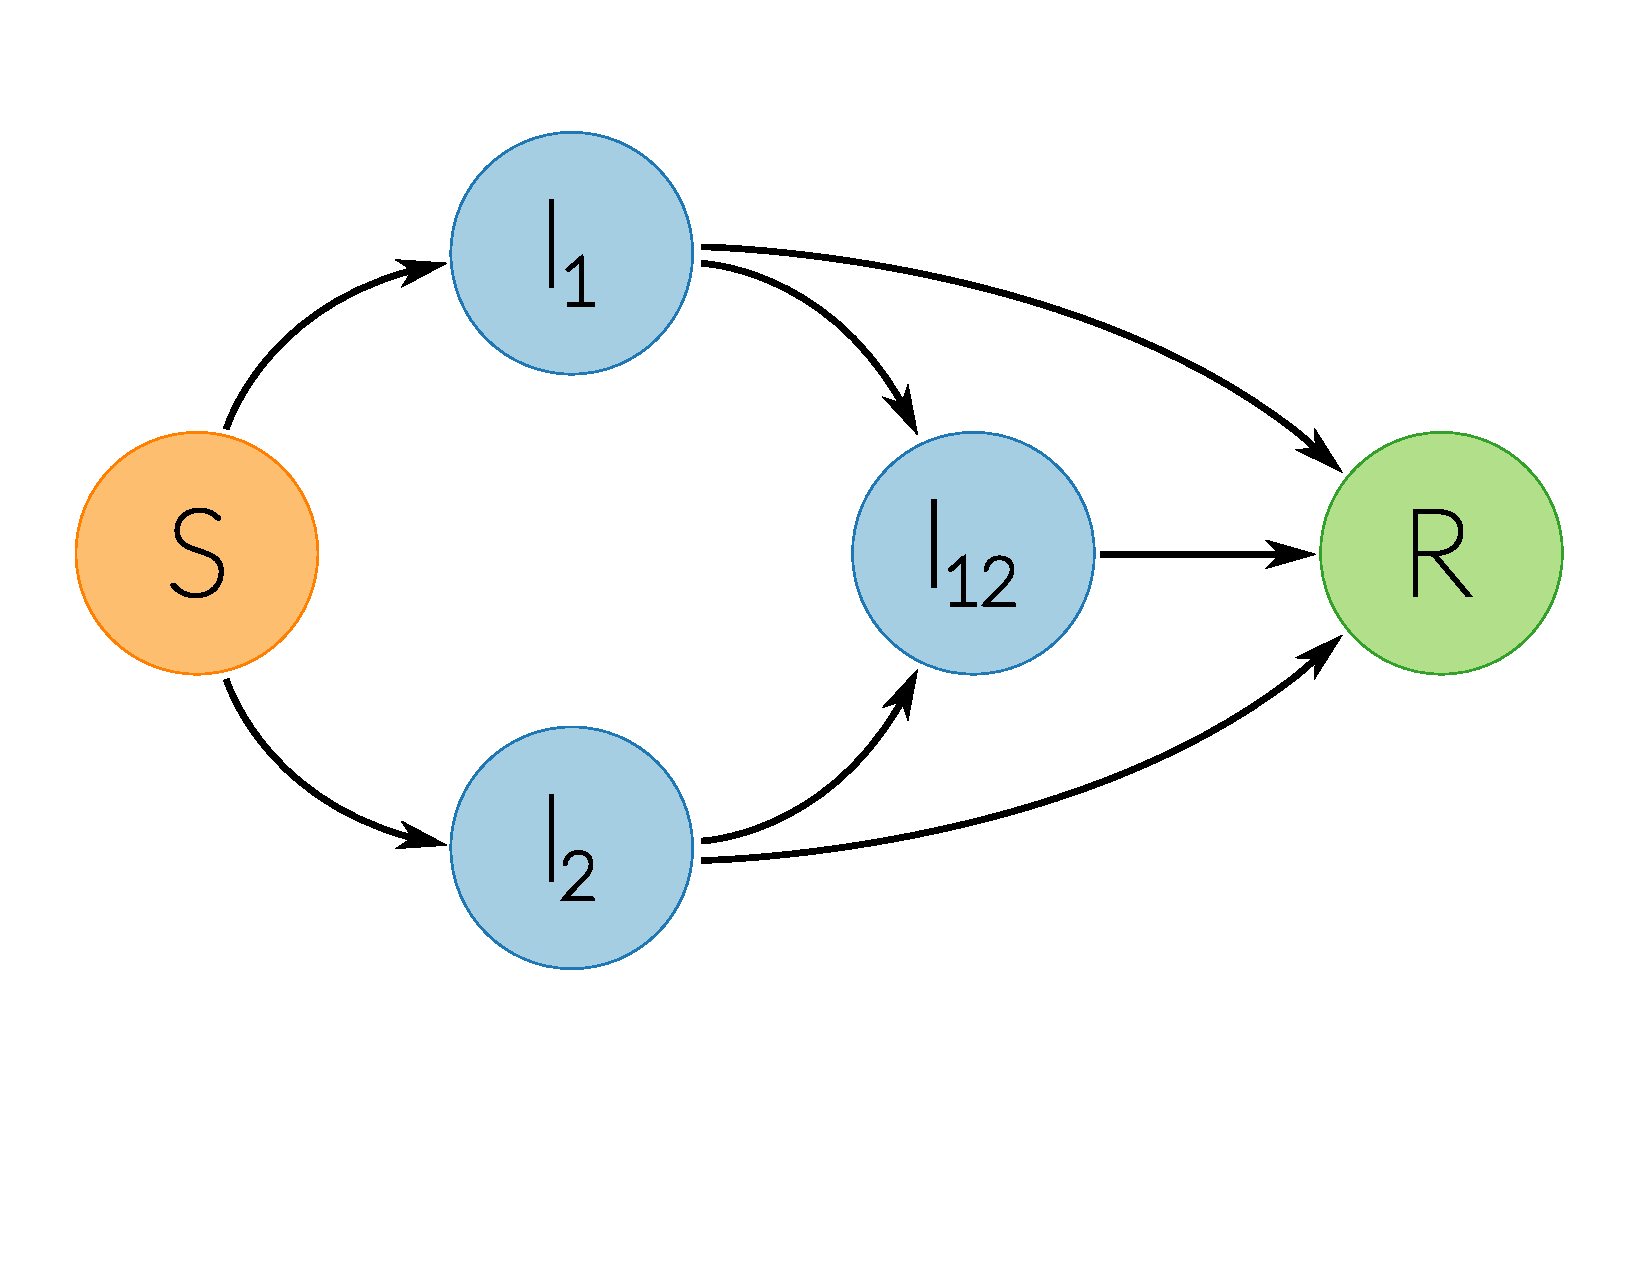
\includegraphics[width=0.4\textwidth]{imgs/SIRoption1.pdf}
  \caption{The SIR model used.}
  \label{f:sir}
\end{figure}


We can now write down the rates of all events. 
I define $I^+_p$ to be the sum of all classes that are infectious with pathogen $p$, for example $I^+_1 = I_1 + I_{12}$. 
Assuming asexual reproduction, that all classes reproduce at the same rate and that individuals are born into the susceptible class we get
\begin{align}
  P\left( S_{nt^\prime} = S_{nt} +1\right) &= b\left( S_{nt}+\sum_q I_{qnt} + R_{nt}\right) 
\end{align}
where $P\left( S_{nt^\prime} = S_{nt} +1\right)$ is the probability that the number of susceptibles in subpopulation $n$ will increase by 1 (a single birth) the short time interval $t$ to $t^\prime$ and $\sum_q I_{qnt}$ is the sum of all infection classes $q \in {1, 2, 12}$.
The rates of death, given a death rate $d$ are given by
\begin{align}
  P\left( S_{nt^\prime} = S_{nt}-1 \right) &= dS_{nt} \\
  P\left( I_{qnt^\prime} = I_{qnt}-1 \right) &= dI_{qnt}\\
  P\left( R_{nt^\prime} = R_{nt}-1 \right) &= dR_{nt}.
\end{align}
Infection of a susceptible with either pathogen 1 or 2, $S \rightarrow I_p$ where $p\in \{1,2\}$, is given by
\begin{align}
  P\left( I_{pnt^\prime} = I_{pnt}+1, S_{nt^\prime} = S_{nt}-1 \right) &= \beta S_{nt}I^+_{pnt},
\end{align}
while coinfection, given a crossimmunity factor $\alpha$, is given by
\begin{align}
  P\left( I_{12,nt^\prime} = I_{12,nt}+1,\: I_{pnt^\prime} = I_{pnt}-1\right) = \alpha\beta I_{nt}I^+_{pnt}.
\end{align}
The probability of migration from colony $m$ (with degree $k_m$) to colony $n$, given a dispersal rate $\lambda$ is given by
\begin{align}
  P\left(S_{nt^\prime}=S_{nt}+1,\: S_{mt^\prime} = S_{mt}-1\right) &= \frac{\lambda S_{mt}}{k_m-1}\\
  P\left(I_{qnt^\prime}=I_{qnt}+1,\: I_{qmt^\prime} = I_{qmt}-1\right) &= \frac{\lambda I_{qmt}}{k_m}\\
  P\left(R_{nt^\prime}=S_{nt}+1,\: R_{mt^\prime} = R_{mt}-1\right) &= \frac{\lambda R_{mt}}{k_m}.
\end{align}
Finally, recovery from any infectious class occurs at a rate $\gamma$
\begin{align}
  P\left( I_{qnt^\prime} = I_{qnt}-1,\: R_{nt^\prime} = R_{nt}+1 \right) &= \gamma I_{qnt}.
\end{align}


\begin{figure}[t]
{\centering 
\subfloat[High $\bar{k}$\label{fig:fullyConnected}]{
  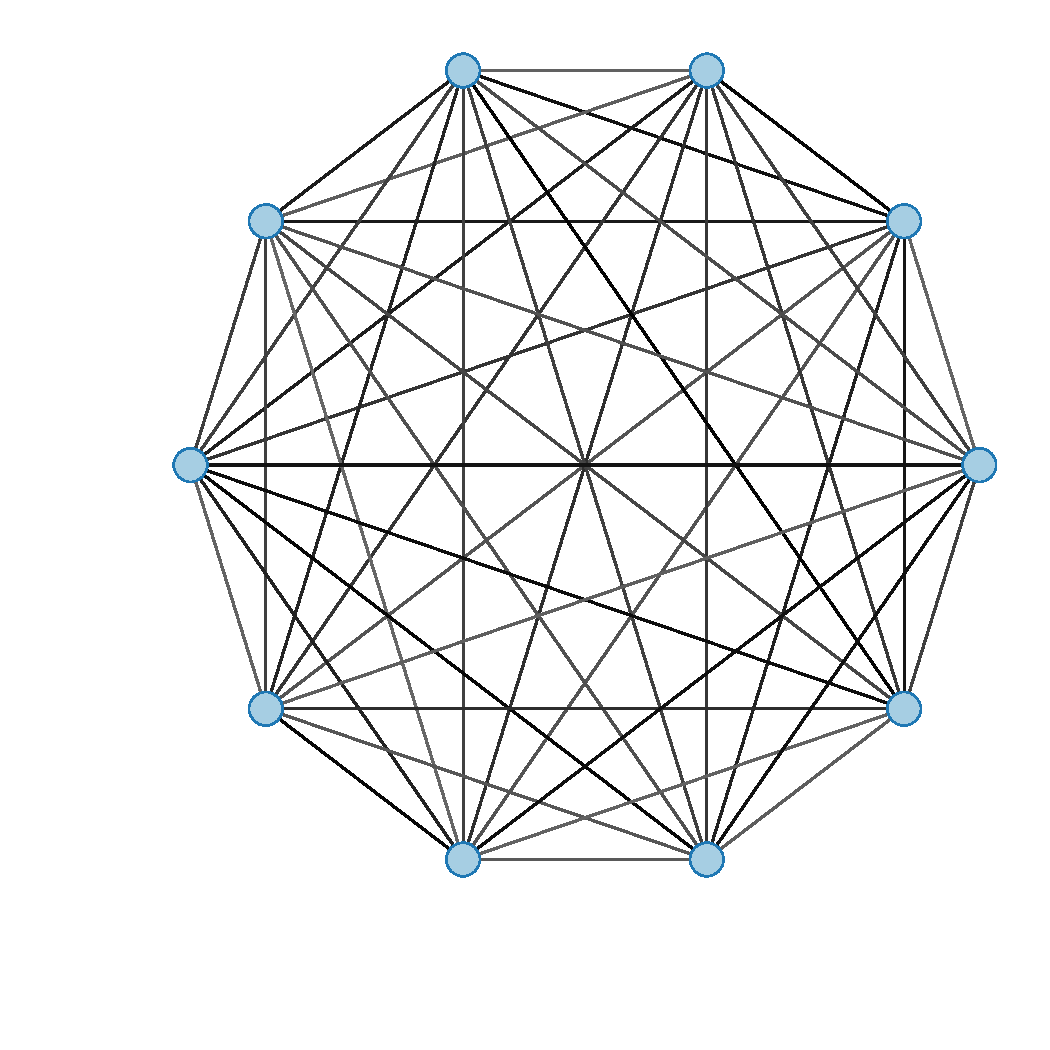
\includegraphics[width=0.45\textwidth]{imgs/fullyConnected.pdf} 
}
\subfloat[Low $\bar{k}$
\label{fig:minimallyConnected}]{
  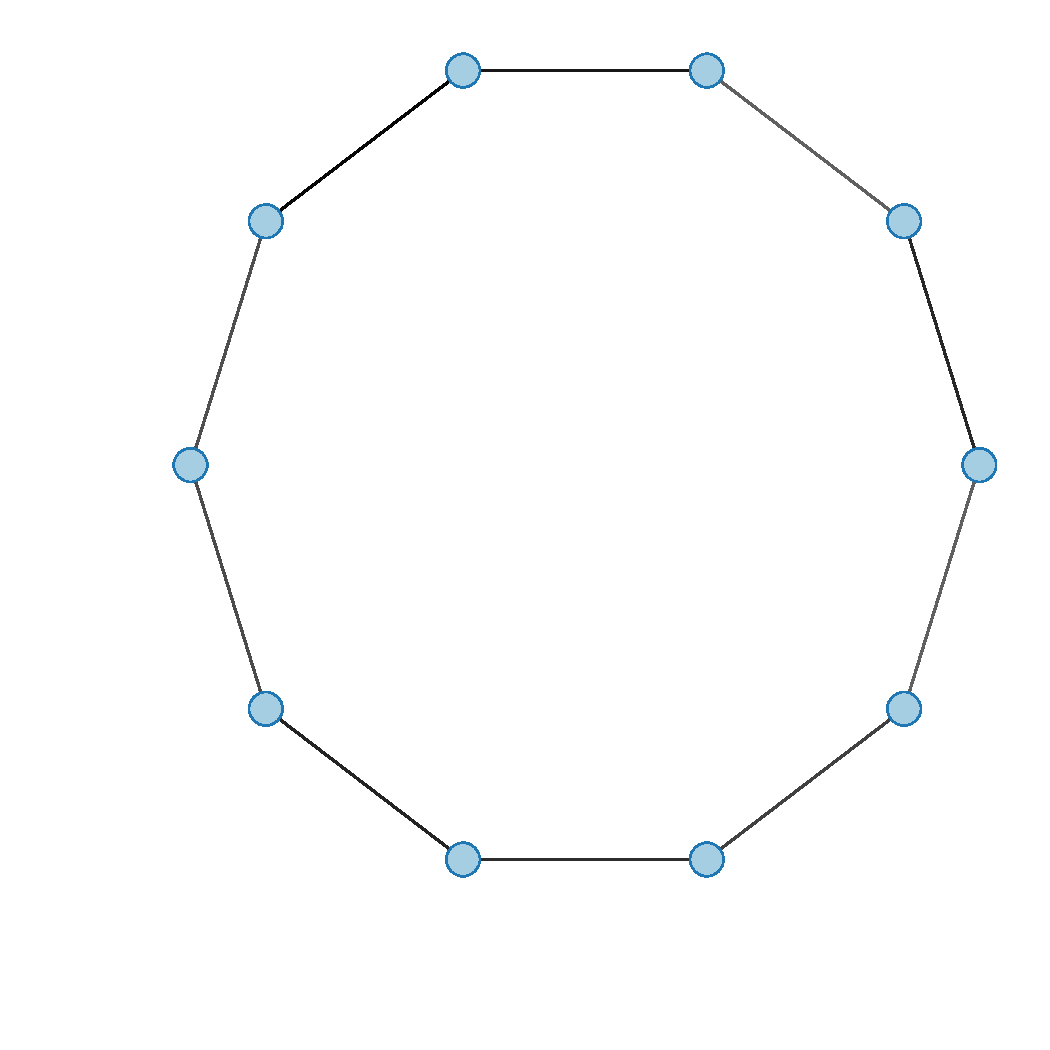
\includegraphics[width=0.45\textwidth]{imgs/minimallyConnected.pdf} 
}
}
\caption[Network topologies used to compare network connectedness]{
The two network topologies used to test whether network connectedness influences a viruses ability to invade. 
Dispersal is held constant between the two topologies.
}
\label{f:net}
\end{figure}















In each simulation the population was seeded with 10 sets of 200 infected individuals of disease 1.
There groups were seeded into randomly selected colonies with replacement.
For each 200 infected individuals added, 200 susceptible individuals were removed to keep starting colony sizes constant. 
Disease 1 was then allowed to spread and reach equilibrium. 
After \ensuremath{3\times 10^{5}} events, 5 individuals infected with disease 2 were added to one colony. 
Visual inspection of preliminary simulations was used to decide on \ensuremath{3\times 10^{5}} as being long enough for the epidemic to reach an equilibrium state.
After another \ensuremath{5\times 10^{5}} events the invasion of disease 2 is considered successful if any individuals with disease 2 still remain.
Again visual inspection of preliminary simulations was used to determine whether this was long enough to be confident that an invading disease 


\subsection{Dispersal}
%%%%%%%%%%%%%%%%%%%%%%%%%%%%%%

The values used for the independant variables are chosen to highlight the affects of these variables. 
Dispersal values are $\lambda = 0.1, 0.01$ and $ 0.001$ dispersals per individual per year. 
$\lambda = 0.1$ relates to individuals moving between colonies on average twice per lifetime. 
Therefore exclusively juvenile dispersal would have dispersal rates similar to this. 
Otherwise it relates to dispersal being a rare event with animals often staying in a colony for many years.
$\lambda = 0.01$ relates to 20\% of individuals dispersing once in their lifetime.
This value is therefore close to male-biased dispersal, with female philopatry. 
Finally, $\lambda = 0.001$ relates to 2\% of individuals dispersing in their lifetime.
This therefore relates to a population that does not habitually disperse.




\subsection{Network structure}
%%%%%%%%%%%%%%%%%%%%%%%%%%%%%%
The network structure is synthetically created to be either fully or minimally connected (See Figure~\ref{f:net}). 
10 subpopulations was selected as a trade off between computation time and a network complicated enough that structure might have an effect. 
This value is artificially small compared to wildlife populations. 



\subsection{Parameter selection}


The fixed parameters used are chosen to roughly reflect realistic wild bat populations. 
The death rate $d$ is set as 0.05 per year giving a generation time of 20 years.
The birth rate $b$ is set to be equal to $d$ so that the population size is stable.
The recovery rate $\gamma$ is set to 1 giving a average infection duration of 1 years. 
This is therefore a long lasting infection but not a chronic infection. 
It is very difficult to directly estimate infection durations in wild populations.
But it seems that these infections might be long lasting \cite{}.

Cross immunity is set to 0.1 so that an individual infected with one disease is 90\% less likely to be infected with another.
This is a rather arbitrary value.
However, the rationale of the model is that the invading species might be a newly speciated strain of the endemic species.
Furthermore, the model assumes complete cross immunity after infection.
Therefore cross immunity is likely to be very strong.

The population size of each subpopulation is set to 3000. 
This is appropriate for many bat species \cite{jones2009pantheria}, especially the large, frugivorous \emph{Pteropodidae} that have been particularly associated with recent zoonotic diseases.


Four values of the transmission rate $\beta$ are used, 0.1, 0.2, 0.3 and 0.4.
All simulations are run under all four transmission rates as this is such a fundamental parameter.
Given the recovery, birth and death rates we can calculate an approximation of $R_0$ that ignores spatial structure.
That is, this is $R_0$ for the local, within-subpopulation dynamics.
Furthermore, it is $R_0$ for the first pathogen; $R_0$ of the invading pathogen will be lower due to competition.
We can calculate that $R_0 \approx \frac{\beta b}{d(d+ \gamma)}$.
For our four values of $\beta = 0.1, 0.2, 0.3, 0.4$ we therefore get $R_0 \approx 13.3, 33.3, 66.6$.
These values are very high in part to again find a reasonable trade off between the number of simulations and the reasonableness of the parameters.
$R_0 \approx 13.3$ is similar to a highly contagious disease such as measles or pertussis. 


For the simulations where an invading pathogen is added to the populations the number of invading pathogens added is set to 10. 
This is a trade off between getting a reasonable proportion of invasions, while still retaining the stochastic nature of invasion.

For simulations studying extinction rates, half of the subpopulation were seeded with each pathogen.
2000 susceptibles and 1000 infected individuals were placed in each subpopulation in order to quickly reach equilibrium.











%%%%%%%%%%%%%%%%%%%%%%%%%%%%%%%%%%%%%%%%%%%%%%%%%%%%%%%%%%%%%%%%%%%%%%%%%%%%%%%%%%%%%%%%%%%%%%%%%%%%%%%%%%%%%%%%%%%%%%%%%%%%%%%%%%%%%%%%%%%%%%%%%%%%%%%%%%%

\clearpage
\section{Results}

%%%%%%%%%%%%%%%%%%%%%%%%%%%%%%%%%%%%%%%%%%%%%%%%%%%%%%%%%%%%%%%%%%%%%%%%%%%%%%%%%%%%%%%%%%%%%%%%%%%%%%%%%%%%%%%%%%%%%%%%%%%%%%%%%%%%%%%%%%%%%%%%%%%%%%%%%%%

















































\begin{knitrout}\footnotesize
\definecolor{shadecolor}{rgb}{0.969, 0.969, 0.969}\color{fgcolor}\begin{figure}[t]

{\centering \subfloat[Dispersal\label{f:invasionPropPlots1}]{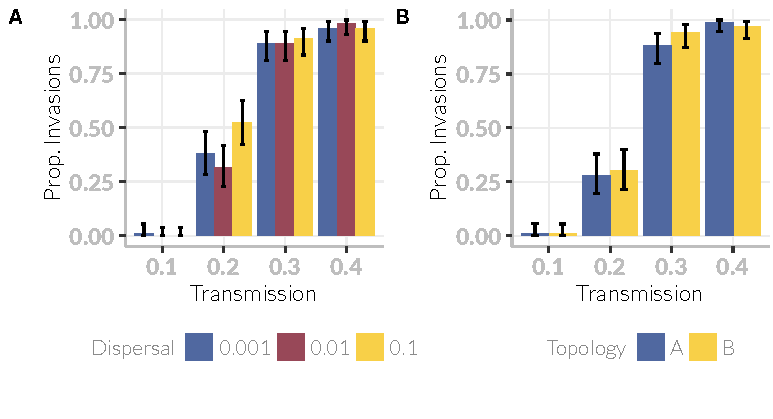
\includegraphics[width=0.45\textwidth]{figure/invasionPropPlots-1} }
\subfloat[Network topology\label{f:invasionPropPlots2}]{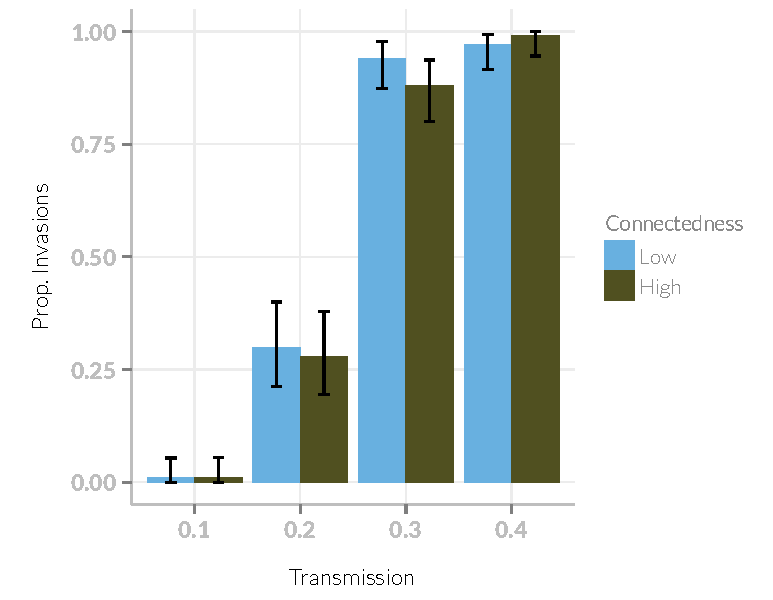
\includegraphics[width=0.45\textwidth]{figure/invasionPropPlots-2} }

}

\caption[The probability of successful invasion]{The probability of successful invasion. 
  For three different transmission rates, the probability of invasion success does not change between different a) dispersal rates or b) network structures. 
  Error bars are 95\% confidence intervals. 
  Other parameters are kept constant at: $N = 10,\, \bar{n} = 3000,\, b = d = 0.05,\, \gamma = 0.1,\, \alpha = 0.1$. 
  When dispersal is varied, the population structure is fully connected. When population structure is varied, $\lambda = 0.01$.}\label{f:invasionPropPlots}
\end{figure}


\end{knitrout}



\subsection{Invasion}


\subsubsection{Dispersal}
%%%%%%%%%%%%%%%%%%%%%%%%%%%%%%


The proportion of invasions was not different across dispersal rates across 1200 simulations run (Figure \ref{f:invasionPropPlots1}).
This was true at all transmission levels ($\chi^2$ test. $\beta = 0.1$: $\chi^2 = 1.98$, $\text{df} = 2$, $p = 0.37$. $\beta = 0.2$: $\chi^2 = 9.44$, $\text{df} = 2$, $p = 0.01$. $\beta = 0.3$: $\chi^2 = 0.29$, $\text{df} = 2$, $p = 0.87$, $\beta = 0.4$: $\chi^2 = 0.83$, $\text{df} = 2$, $p = 0.66$).


\subsubsection{Network structure}
%%%%%%%%%%%%%%%%%%%%%%%%%%%%%%

I ran 800 simulations over 4 transmission values ($\beta = $ 0.1, 0.2, 0.3, 0.4).
The proportion of invasions was not different between highly connected and largely unconnected metapopulations (Figure~\ref{f:invasionPropPlots2}). 
This was true at all transmission levels ($\chi^2$ test. $\beta = 0.1$: $\chi^2 = \ensuremath{5.23\times 10^{-31}}$, $\text{df} = 1$, $p = 1$. $\beta = 0.2$: $\chi^2 = 0.02$, $\text{df} = 1$, $p = 0.88$. $\beta = 0.3$: $\chi^2 = 1.53$, $\text{df} = 1$, $p = 0.22$. $\beta = 0.4$: $\chi^2 = 0.26$, $\text{df} = 1$, $p = 0.61$).

 
\subsection{Transmission}
%%%%%%%%%%%%%%%%%%%%%%%%%%

Inline with theory, increasing the transmission rate increased the probability of invasion (Figure~\ref{f:invasionPropPlots1}--\ref{f:invasionPropPlots2}).
This is true for all three dispersal values ($\chi^2$ test. $\lambda = 0.001$: $\chi^2 = 243.56$, $\text{df} = 3$, $p = \ensuremath{1.62\times 10^{-52}}$. $\lambda = 0.01$: $\chi^2 = 265.4$, $\text{df} = 3$, $p = \ensuremath{3.05\times 10^{-57}}$. $\lambda = 0.1$: $\chi^2 = 244.95$, $\text{df} = 3$, $p = \ensuremath{8.1\times 10^{-53}}$) and both network structures ($\chi^2$ test. Fully connected: $\chi^2 = 267.3$, $\text{df} = 3$, $p = \ensuremath{1.18\times 10^{-57}}$. Minimally connected: $\chi^2 =  267.3$, $\text{df} = 3$, $p = \ensuremath{1.18\times 10^{-57}}$).



%%%%%%%%%%%%%%%%%%%%%%%%%%%%%%%%%%%%%%%%%%%%%%%%%%%%%%%%%%%%%%%%%%%%%%%%%%%%%%%%%%%%%%%%%%%%%%%%%%%%%%%%%%%%%%%%%%%%%%%%%%%%%%%%%%%%%%%%%%%%%%%%%%%%%%%%%%%

\clearpage
\section{Discussion}

%%%%%%%%%%%%%%%%%%%%%%%%%%%%%%%%%%%%%%%%%%%%%%%%%%%%%%%%%%%%%%%%%%%%%%%%%%%%%%%%%%%%%%%%%%%%%%%%%%%%%%%%%%%%%%%%%%%%%%%%%%%%%%%%%%%%%%%%%%%%%%%%%%%%%%%%%%%

\subsection{Restate the gap and the main result}

Empirical studies on the role of population structure on the are equivocal and cannot examine the specific mechanisms by which pathogen communities are created and maintained.
I have used mechanistic, metapopulation models to test whether increased population structure can promote pathogen richness by facilitating invasion of new pathogens.



\subsection{Link results to consequences}

\subsubsection{Population structure does not affect pathogen richness}

Probably because dynamics are dominated by local processes.
This goes against many predictions that increasing $R_0$ increases pathogen richness.
Further work could examine reduced col  ony sizes to test when global structure become more important.
Measures of population structure should not be used to predict zoonotic potential.

\subsubsection{Dispersal does not affect pathogen richness}



\subsubsection{Network connectedness does not affect pathogen richness}

This is in direct contrast to \cite{campos2006pathogen}. 
However, the model in \cite{campos2006pathogen} is a contact network, so increasing the connectedness increases the chance of succesful transmission events for the first few transmission generations.
This lends support to the idea that I found now affect of connectedness due to the dominance of local dynamics.

Network connectedness can be seen as a function of average dispersal distance, density and colony size.
A high density species with small colony sizes must have colonies relatively close together.
Therefore colonies would be more likely to be connected for a given dispersal distance. 


\subsection{Discuss assumptions}

\subsubsection{Complete cross-immunity}

I have assumed that once recovered, individuals are immune to both pathogens. 
Furthermore, when a coinfected individual recovers from one pathogen, it immediately recovers from the other as well.
This is probably a fairly reasonable assumption given that I am modelling a newly evolved strain.
However, further work could relax this assumption using a model similar to \cite{poletto2015characterising} which contains additional classes for `infected with pathogen one, immune to pathogen two' and `infected with pathogen two, immune to pathogen one'.
The model here was formulated such that the study of systems with greater than two pathogens is still computationally feasible while a model such as used in \cite{poletto2015characterising} contains $3^\rho$ classes for a system with $\rho$ pathogen species.
This quickly becomes computationally restrictive.

\subsubsection{Identical strains}

Many papers on pathogen richness have focussed on the evolution of pathogen traits and have considered a trade off between transmission rate and virulence \cite{nowak1994superinfection, nowak1994superinfection} or infectious period \cite{poletto2013host}.
However, here we are interested in host traits.
Therefore we have assumed that pathogen strains are identical.
It is clear however that there are a number of factors that affect pathogen richness and our focus on host population structure does not imply that pathogen traits are not important.



%%%%%%%%%%%%%%%%%%%%%%%%%%%%%%%%%%%%%%%%%%%%%%%%%%%%%%%%%%%%%%%%%%%%%%%%%%%%%%%%%%%%%%%%%%%%%%%%%%%%%%%%%%%%%%%%%%%%%%%%%%%%%%%%%%%%%%%%%%%%%%%%%%%%%%%%%%%

\clearpage
\section{Appendix}

%%%%%%%%%%%%%%%%%%%%%%%%%%%%%%%%%%%%%%%%%%%%%%%%%%%%%%%%%%%%%%%%%%%%%%%%%%%%%%%%%%%%%%%%%%%%%%%%%%%%%%%%%%%%%%%%%%%%%%%%%%%%%%%%%%%%%%%%%%%%%%%%%%%%%%%%%%%

\begin{table}[b!]

\begin{tabular}{lp{5.7cm}p{4.3cm}l}
 & Explanation & Units&Value\\
\hline
$S$ & Susceptible individuals &&\\
$I_q$ & Infectious with diseases $q$ &&\\
$I^+_p$ & Sum of classes infected with pathogen $p$ &\\
$N$ & Number of colonies&& 10\\
$\bar{n}$ & Mean colony starting size && 3000\\
$\beta$ & Transmission rate & Transmission events per year per individual& 2, 5, 10\\
$\gamma$ & Recovery rate & Recovery events per year per individual. & 1\\
$\lambda$ & Dispersal & Dispersal events per day per individual& 0.001--0.1\\
$b$ & Birth rate & Births per year per individual& 0.05\\
$d$ & Death rate & Deaths per year per individual & 0.05\\
$d_I$ & Infectious death rate & Additional deaths per day per individual&\\
$\rho$ & No. pathogens && 2\\
$p$ &  Pathogen index i.e. $p\in\{1,2\}$ for pathogens 1 and 2 & &\\
$q$ & Disease class i.e., $q\in\{1,2,12\}$&\\
$\mathcal{V}$ & Neighbourhood of a node &&\\
$t, t^\prime$ & Time and time plus waiting time i.e., $t+\delta$ & Days&\\
$k_i$ & Degree of node $i$ &&\\
$\delta$ & Waiting time until next event & Days&\\
$\alpha$ & Cross immunity & Proportion& 0.1\\
$n, m$ & Colony index &&\\
$\bm{A}_{mn}$ & Adjacency matrix. & Distance &\\
$\mu$ & Maximum distance for edge to exist & km& 40, 100\\
$\sigma$ & Invading pathogen seed size & & 10\\
$r_i$ & The rate that event $i$ occurs. & Days$^{-1}$&\\
&&&\\
\end{tabular}
\caption{All symbols used.}
\label{t:params}
\end{table}




